\documentclass[12pt]{article}

\usepackage[left=2.5cm,right=2.5cm,top=2.5cm,bottom=2.5cm]{geometry}
\usepackage{graphicx}
\usepackage[dvipsnames]{xcolor}
\usepackage{tikz}
\input{tikz/interfacepoint.tikzstyles}
\usepackage{tikz-cd}
\usepackage{tikz-qtree}
\usetikzlibrary{shapes,backgrounds,calc,arrows}
\usepackage{microtype}

\usepackage[setpagesize=false, colorlinks=true,urlcolor=red,pdftitle={Simplicial Coalgebras for Concurrent Regular Languages},pdfauthor={Hessel Sieburgh}]{hyperref}
\frenchspacing
\setlength\parindent{0pt}

\usepackage{amsmath}
\usepackage[utf8]{inputenc}
\usepackage{amsfonts}
\usepackage{amssymb}
\usepackage{amsthm}
\usepackage{theoremref}
%\usepackage{cleveref}
\usepackage{float}

\usepackage{doi}

\makeatletter
\renewcommand{\th@definition}{%
  \normalfont
  \thm@preskip 18pt \relax
  \thm@postskip 18pt \relax
}
\makeatother

\makeatletter
\renewcommand{\th@plain}{
  \thm@preskip 18pt \relax
  \thm@postskip 18pt \relax
}
\makeatother

\newtheorem{theorem}{Theorem}[section]
\newtheorem{lemma}[theorem]{Lemma}
\newtheorem{prop}[theorem]{Proposition}
\newtheorem{corollary}[theorem]{Corollary}

\theoremstyle{definition}
\newtheorem{definition}[theorem]{Definition}
\newtheorem{remark}[theorem]{Remark}
\newtheorem{example}[theorem]{Example}

\usepackage{bbm}
\usepackage{csquotes}
\usepackage{mathtools}
\usepackage{parskip}
\usepackage{mathtools}
\usepackage{mathdots}
\usepackage{stmaryrd}
\newcommand{\defeq}{\vcentcolon=}
\newcommand{\eqdef}{=\vcentcolon}

\DeclareMathOperator{\Ima}{Im}
\DeclareMathOperator{\sech}{sech}
\renewcommand{\P}{\mathcal{P}}
\newcommand{\R}{\mathbb{R}}
\newcommand{\C}{\mathbb{C}}
\newcommand{\N}{\mathbb{N}}
\newcommand{\E}[1]{\mathbb{E}\{#1\}}
\newcommand{\Q}{\mathbb Q}
\newcommand{\Z}{\mathbb{Z}}
\newcommand{\1}{\mathbbm{1}}
\newcommand{\ua}{\nearrow}
\newcommand{\da}{\searrow}
\newcommand{\eps}{\varepsilon}
\newcommand{\dx}{\mathrm{d}x}
\newcommand{\B}{\mathcal{B}}
\newcommand{\F}{\mathcal{F}}
\newcommand{\T}{\mathbb{T}}
\newcommand{\V}{\mathcal{V}}
\newcommand{\U}{\mathcal{U}}
\newcommand{\id}{\text{id}}
\newcommand{\I}{\mathcal{I}}
\newcommand{\A}{\mathcal{A}}
\newcommand{\J}{\mathcal{J}}
\newcommand{\G}{\mathcal{G}}
\renewcommand{\L}{\mathcal{L}}
\newcommand{\specepsilon}{\mathcal{E}}
\newcommand{\M}{\mathcal{M}}
\newcommand{\II}{\textbf{II}}
\newcommand{\bigo}{\mathcal{O}}
\renewcommand{\H}{\mathcal{H}}
\newcommand{\finP}{\mathcal{P}_{\omega}}
\newcommand{\Set}{\mathbf{Set}}
\newcommand{\JSL}{\text{JSL}}
\newcommand{\seq}{;}
\newcommand{\pred}{\text{pred}}
\newcommand{\textover}[2]{\mathrel{\overset{\makebox[0pt]{\mbox{\normalfont\tiny\sffamily #1}}}{#2}}}
\newcommand{\beh}{\overline{c}}

%\setlength{\parskip}{1em}

\begin{document}
\thispagestyle{empty}


\includegraphics{logoleiden}

\vspace{-2.5cm}\hfill \begin{huge}\textbf{Opleiding Informatica}\end{huge}

\vspace{5cm}
\begin{Large}
\hfill Simplicial Coalgebras

\vspace*{3mm}

\hfill for Concurrent Regular Languages

\vspace*{14mm}

\hfill Hessel Sieburgh
\end{Large}

\vspace*{6.0cm}

\begin{large}

Supervisors:\\
Henning Basold \& 
Marton Hablicsek


\vspace*{2.8cm}
BACHELOR THESIS

\vspace*{5mm}
Leiden Institute of Advanced Computer Science (LIACS)\\
\href{www.liacs.leidenuniv.nl}{\underline{\texttt{www.liacs.leidenuniv.nl}}}\hfill 01/07/2025
\end{large}

\newpage


\begin{abstract}
\noindent
Regular expressions give an easy way to express regular languages, and through Kleene's theorem we know the regular languages they describe are exactly equal to the ones modelled by deterministic finite automata. These automata give a very efficient way to parse strings, search through data, check for patterns etc. But these regular languages only contain strings of characters, given by sequential composition. In practice machines, software, biology, and other forms of data exhibit concurrent behaviour. Such as parallel computing, manufacturing with multiple steps which aren't directly dependent, or cellular activity in organisms.

In contrast to regular languages, a model for these concurrent languages, together with expressions, hasn't been found yet. Previous attempts have been made but they haven't been as useful as wanted. We think the main problem with the previous approaches have been the conflation of structure with behaviour, transitions in the model were restricted by the form of the state space.

For this problem we first propose a new type of dependency graph called ranked hypergraphs. These are directed acyclic hypergraphs which have root and output interfaces that give control over dependencies and the defined sequential composition is associative up to isomorphism.

Because of the interfaces there is a generator of graphs of depth 1. Which means that in these graphs there isn't a path longer than 1 edge. We can inductively split up any graph into these pieces, which lets them serve as building blocks for all ranked hypergraphs.

As structure for these graphs we define a simplicial set containing them. Finally, a coalgebra is used to define a transition and acceptance system for these states, mirroring classical automata by splitting up graphs into their building blocks.
\end{abstract}

\bigskip
\newpage
\thispagestyle{empty}
\tableofcontents
\thispagestyle{empty}

\clearpage
\setcounter{page}{1}

\section{Introduction} \label{introduction}
Finite automata and regular languages form the foundation of classical formal language theory. Deterministic finite automata (DFA) provide a simple and elegant model for accepting regular languages, with Kleene's theorem stating their equivalence to regular expressions. In this setting, words are sequential compositions from single letters in an alphabet, and state transitions are deterministic.

However, many systems exhibit concurrent behaviour, where actions occur in parallel with complex dependencies. In a previous attempt to model this behaviour, higher-dimensional automata (HDA) were proposed. In HDA, concurrent actions are modelled using paths through hypercubes. But this combination of structure and behaviour is constricting and leads to just a small set of described languages. The missing part in particular is a parallel equivalent to the Kleene star operation.

In this thesis, we develop an approach to model concurrent regular languages which separates structure from behaviour: simplicial coalgebras over ranked hypergraphs. 

We introduce ranked hypergraphs with interfaces that allow associative composition up to renaming. The interfaces give a way to connect dependencies. This composition allows for a generator which consists of graphs of depth 1. 

The generator allows for piece-by-piece parsing of a graph. Mirroring how finite automata parse a word character by character. With the alphabet being the generator.

We will first introduce the necessary background on simplicial sets, subobject identifiers and coalgebras. We then formalize ranked hypergraphs and their compositions, describe the simplicial structure, and finally define the coalgebraic behaviour function which gives the parsing semantics.

\subsection{Related Work}

\paragraph{Interface pomsets}
In discrete finite automata (DFA) over an alphabet $\Sigma$ we work with single characters, which when sequentially composed build the words of languages. But in concurrent settings we need actions which have multiple events that can be parallel, dependent, weakly dependent, etcetera. But to be useful they also need a structure that allows composition, and most ideally a generator.

For this, interface pomsets were introduced \cite{ipomsets2024}. 

\begin{definition}{\cite{ipomsets2024}}
    An \emph{ipomset} (over an alphabet $\Sigma$) is a structure $(P, <, \dashrightarrow, S, T, \lambda)$ consisting of the following:
    \begin{itemize}
        \item a finite set $P$ of \emph{events},
        \item a strict partial order (i.e., asymmetric, transitive, irreflexive) $<\, \subseteq P\times P$ called the precedence order,
        \item a strict partial order $\dashrightarrow\,\subseteq P\times P$ called the \emph{event order},
        \item a subset $S\subseteq P$ called the \emph{source set} of \emph{sources},
        \item a subset $T\subseteq P$ called the \emph{target set} of \emph{targets},
        \item a \emph{labelling} map $\lambda: P\to \Sigma$.
    \end{itemize}
\end{definition}

Intuitively we understand the precedence order, if $a<b$ then $a$ must end before $b$ begins. The event order is a weaker notion which is necessary for sequential composition. The source and target sets are also used for composition, we can only \emph{glue} two ipomsets $P$ and $Q$ together if $T_P \cong S_Q$.

We identify a couple of important types of ipomsets. Namely, an ipomset $(P,<,\dashrightarrow, S, T, \lambda)$ is:

\begin{itemize}
    \item \emph{discrete} if $<$ is empty,
    \item a \emph{conclist} (short for `concurrency list') if it is discrete and $S=T=\varnothing$,
    \item a \emph{starter} if it is discrete and $T = P$,
    \item a \emph{terminator} if it is discrete and $S = P$, and
    \item an \emph{identity} if it is both a starter and a terminator.
\end{itemize}

An \emph{isomorphism} of ipomsets $P$ and $Q$ is a bijection $f: P\to Q$ such that:
\begin{enumerate}
    \item $f(S_P) = S_Q$, $f(T_P) = T_Q$, $\lambda_Q\circ f = \lambda_P$,
    \item $f(x) <_Q f(y) \iff x <_P y$, and
    \item $x \nless_P y$ and $y\nless_P x$ imply that $x\dashrightarrow_P y \iff f(x)\dashrightarrow_Q f(y)$.
\end{enumerate}

\begin{prop}
    Isomorphism classes of ipomsets form a category $\mathrm{iiPoms}_{\simeq}$.
    \begin{itemize}
        \item objects are isomorphism classes of conclists,
        \item morphisms in $\mathrm{iiPoms}_{\simeq}(U,V)$ are isomorphism classes of ipomsets $P$ with $S_P = U$ and $T_P = V$,
        \item composition of morphisms is gluing, and
        \item identities are identity ipomsets, i.e. $(U, \varnothing, \dashrightarrow, U, U, \lambda)\in\mathrm{iiPoms}_{\simeq}(U,U)$.
    \end{itemize}
\end{prop}

Finally, let $\mathit{\Bar{\Omega}_{\simeq}}$ be the directed multigraph given as follows:
\begin{itemize}
    \item Vertices are objects of $\mathrm{iiPoms}_{\simeq}$.
    \item Edges in $\mathit{\Bar{\Omega}_{\simeq}}$ are morphisms in $\mathrm{iiPoms}_{\simeq}(U,V)$
\end{itemize}

\begin{corollary}[\cite{ipomsets2024}]
    The category $\mathrm{iiPoms}_{\simeq}$ is generated by the directed multigraph $\mathit{\Bar{\Omega}_{\simeq}}$ using gluing composition under the identities \cite[equation. (2)]{ipomsets2024}.
\end{corollary}

The concept of discreteness in starters and terminators inspired the generator of ranked hypergraphs, described in \thref{thm_generator}. In our case, if an edge has a predecessor then the action of that predecessor has to happen first. No precedence order would therefore translate to all edges having no predecessors. Therefore giving directed graphs of depth 1.

\paragraph{Higher Dimensional Automata}
Higher Dimensional Automata (HDA) have been proposed as an analogue of DFA for modelling concurrent languages \cite{Pra91, vG91}. An HDA is a \emph{precubical set} with start and end points. Which means its states have the structure of hypercubes, with direction over its edges inducing direction for cells of all dimensions.
\begin{figure}[H]\label{fig:HDA_paths}
    \centering
    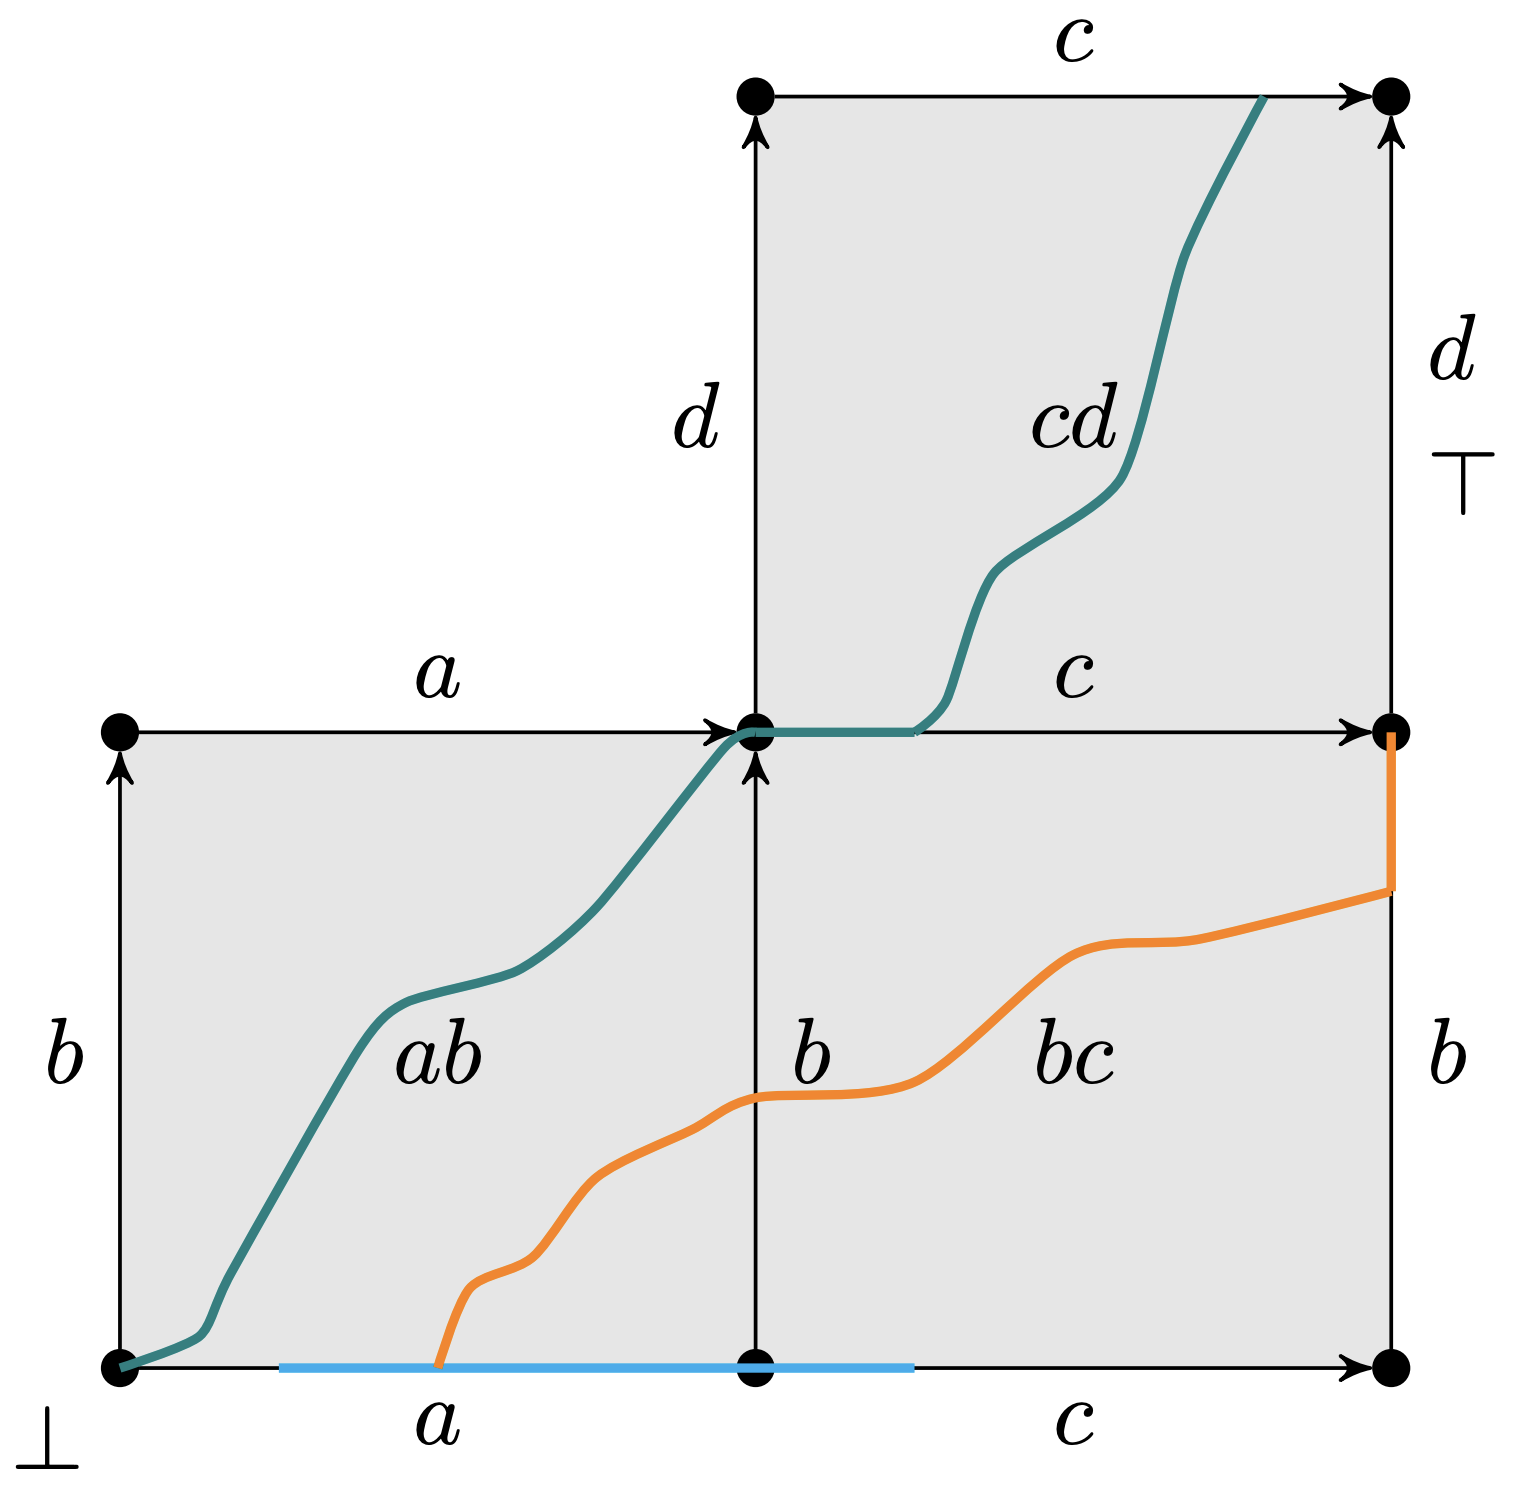
\includegraphics[width=0.5\linewidth]{HDA_paths.png}
    \caption{Paths in a HDA}
\end{figure}

A Kleene theorem was found for these automata by Fahrenberg et. al. \cite{Fahr_2024} which proves the languages HDA define are exactly the rational subsumption-closed sets of finite interval pomsets. One of the limitations of this is that the rational operations used by Fahrenberg et. al. don't include a `parallel Kleene star' but only a binary (therefore finite) parallel composition. Thus severely restricting the description of concurrency by this class of languages.
\newpage
\section{Background}
\subsection{Preliminaries}
This thesis assumes basic knowledge of and experience with automata theory and category theory. A good starting point for automata would be chapters 2-3 of \emph{Introduction to Languages and the Theory of Computation} by John C. Martin \cite{Martin_2011}. For category theory I would recommend the classic book \emph{Categories for the Working Mathematician} \cite{MacLane1998}.

\subsection{Semilattices}
\begin{definition}
    Let $P$ be a partially ordered set (poset), the \emph{join} (or least upper bound) is a binary operator $\vee$ such that for all $x,y,z\in P$:
    \begin{itemize}
        \item $x\leq x\vee y$,
        \item if $x\leq a$ and $y\leq a$ then $x\vee y\leq a$.
    \end{itemize}

    the \emph{meet} (or greatest lower bound) is a binary operator $\wedge$ such that for all $x,y,z\in P$:
        \begin{itemize}
        \item $x\wedge y\leq x$,
        \item if $z\leq x$ and $z\leq y$ then $z\leq x\wedge y$.
    \end{itemize}
\end{definition}

\begin{definition}
    A \emph{join-semilattice} is a triple $(A, \vee, \bot)$ consisting of
    \begin{itemize}
        \item A partially ordered set $A$,
        \item A binary join $\vee: A\times A \to A$ which is commutative, associative, and idempotent: $a\vee a = a$,
        \item A unit $\bot$ such that $a \vee\bot = a$.
    \end{itemize}

    The collection of all join-semilattices forms a category JSL.

    A \emph{meet-semilattice} is the same as a join-semilattice, except we have as operator a meet instead of a join.

    An object that is both a meet-, and a join-semilattice is called a \emph{lattice}. 
\end{definition}

\begin{definition}
    Let $X$ be a set. Let $\finP(X)$ be the set of finite subsets of $X$, then $(\finP(X), \cup, \varnothing)$ is a JSL.
\end{definition}

\begin{definition}
    The free join-semilattice on a set $X$ is the unique JSL $F(X)$ together with a function $\eta: X\to F(X)$ such that for all $A\in\JSL$, $f: X \to A$ there exists a unique JSL morphism $\hat{f}: F(X)\to A$ such that the following diagram commutes:
    \begin{center}
        \begin{tikzcd}
              X \arrow[d,"\eta"]\arrow[r,"f"] & A  \\
              F(X) \arrow[ur, swap, "\hat{f}"]
        \end{tikzcd}
    \end{center}
\end{definition}

This definition is a special case of the more general notion of a free object \cite{joy_of_cats_2009}.

\begin{lemma}\thlabel{lem:free_jsl}
    Let $X\in \Set$, $\finP(X)$ is the free JSL on $X$.
\end{lemma}

\begin{proof}
    Take $\eta(x) = \{x\}$. Let $A$ be a join-semilattice, $f: X \to A$ a function and let $\hat{f}(\{x_1, \dots, x_n\}) = f(x_1)\vee \dots \vee f(x_n)$.\

    Then $(\hat{f}\circ \eta)(x) = \hat{f}(\{x\}) = f(x)$. And thus the finite powerset is the unique free JSL.
\end{proof}

\begin{definition}
    A Heyting algebra H is a lattice together with the operation of implication $\Rightarrow: H\times H \to H$ which for all $x,y,z\in H$ satisfies:
    \[
        x\wedge y \leq z \iff x\leq y\Rightarrow z
    \]
\end{definition}

Moreover, a Heyting algebra where the \emph{principle of excluded middle} holds, which states every proposition is either true or false, is a Boolean algebra. When writing $\vdash$ for $\leq$ you get precisely the classical notion of propositional logic.

\subsection{Presheaves}
\begin{definition}
    Let $C$,$D$ be categories, and $F,G: C\to D$ be functors. Then a \emph{natural transformation} $\mu: F\Rightarrow G$ from $F$ to $G$ is a family of morphisms such that:
    \begin{enumerate}
        \item for all $x\in C$ there exists a morphism $\mu_x: F(x)\to G(x)$ called the component at $x$
        \item for all $x,y\in C$ and all morphisms $f: x\to y$ the following diagram commutes:
        \begin{equation}\label{eq:nat-trans}
            \begin{tikzcd}
                F(x) \arrow{r}{F(f)} \arrow{d}{\mu_x} & F(y) \arrow{d}{\mu_y} \\
                G(x) \arrow{r}{G(f)} & G(y)
            \end{tikzcd}
        \end{equation}
    \end{enumerate}
\end{definition}

\begin{definition}
    Let $C$ be a category, a \emph{presheaf} is a functor \[
        F: C^{op}\to \Set
    \]
    The collection of all presheaves on a category forms a category with as morphisms the natural transformations between the presheaves.
\end{definition}

\subsection{Simplicial sets}
\begin{definition}
    The simplex category $\Delta$ has as objects
    \[
        [n] = \{0 < 1 < \dots < n\}
    \]
    and as morphisms the order-preserving functions between them.

    For all $n\in\N$, $i\in [n]$ we define the coface map $\delta^n_i: [n-1]\to [n]$ as the injective order preserving map which has $(\delta^n_i)^{-1}(i) = \varnothing$. So the map 'misses' $i$ and all other elements of $[n]$ are 'hit'.

    For all $n\in\N$, $i\in [n]$ we define the coface map $\sigma^n_i: [n-1]\to [n]$ as the surjective order preserving map which has $|(\sigma^n_i)^{-1}(i)| = 2$, $|(\sigma^n_i)^{-1}(j)| = 1$ $\forall j\neq i$. So the map 'hits' $i$ twice, and all other $j$ once.

    All morphisms of $\Delta$ are generated from the coface and codegeneracy maps.
\end{definition}

\textit{Notation: } $\delta_i^n$, $\sigma_i^n$ and so on, are just referred to as $\delta_i$, $\sigma_i$ etc. As the exact $n$ is not necessary for most applications. 

\begin{definition}
    A \emph{simplicial set} is a presheaf on \( \Delta \), which means a simplicial set is a functor
    \[
    X \colon \Delta^{\mathrm{op}} \to \Set
    \]
    
    Thus, a simplicial set \( X \) assigns to each \( [n] \in \Delta \) a set \( X_n = X([n]) \) of \emph{n-simplices}, and to each morphism \( \theta \colon [m] \to [n] \), a function \( X(\theta) \colon X_n \to X_m \).
    
    In particular, we have $X(\delta_i) = d_i$ where $d_i: X_n\to X_{n-1}$ omits the $i$-th element from an $n$-simplex. And $X(\sigma_i) = s_i$ where $s_i: X_n \to X_{n+1}$ repeats the $i$-th element in the simplex.
    
    These satisfy the \emph{simplicial identities}:
    \[
    \begin{aligned}
    d_i d_j &= d_{j-1} d_i && \text{if } i < j, \\
    s_i s_j &= s_{j+1} s_i && \text{if } i \leq j, \\
    d_i s_j &=
    \begin{cases}
    s_{j-1} d_i & \text{if } i < j, \\
    \mathrm{id} & \text{if } i = j \text{ or } i = j+1, \\
    s_j d_{i-1} & \text{if } i > j+1.
    \end{cases}
    \end{aligned}
    \]

    The presheaf category of simplicial sets is called $\mathrm{sSet}$ and its natural transformations the \emph{simplicial morphisms}.
    
    Given a collection of sets $S = S_0 \sqcup S_1 \sqcup \dots$ and functions $d_i: S_n\to S_{n-1}$, $s_i: S_n \to S_{n+1}$ satisfying the simplicial identities there is a unique simplicial set which has the same face and degeneracy maps.
\end{definition}

\begin{lemma}
    Let $X, Y\in \mathrm{sSet}$, a collection of morphisms $f_0: X_0\to Y_0, f_1: X_1\to Y_1, \dots$ is a simplicial morphism if and only if the following diagrams commute.
    \[
        \begin{tikzcd}
        X_n \arrow{r}{d_i^X} \arrow{d}{f_n} & X_{n-1} \arrow{d}{f_{n-1}} \\
        Y_n \arrow{r}{d_i^Y} & Y_{n-1}
        \end{tikzcd}
        \quad
        \begin{tikzcd}
        X \arrow{r}{s_j^X} \arrow{d}{f_n} & X_{n+1} \arrow{d}{f_{n+1}} \\
        Y_n \arrow{r}{s_j^Y} & Y_{n+1}
        \end{tikzcd}
    \]
\end{lemma}

\begin{proof}
    Given that $\delta_i$, $\sigma_i$ generate the morphisms in $\Delta$, diagram \ref{eq:nat-trans} automatically commutes for all $f$ if it does so for $\delta$ and $\sigma$.
\end{proof}

\begin{definition}
    Let $U$ be a poset, denote by $U^{\rhd}$ the poset $U$ with a new maximal element added. On $\Delta$ this gives $[n]^{\rhd} \cong [n+1]$. 

    This gives a functor $\uparrow: \mathrm{sSet}\to \mathrm{sSet}$ by $\uparrow X = X\circ (-)^{\rhd}$. Then for $x\in X_n$ and $f:X\to \uparrow X$ we have $f(x)\in X_{n+1}$.
\end{definition}

\subsection{Subobject Classifiers}
\begin{definition}
    Let $f, g$ be morphisms defined by
    \begin{center}
        \begin{tikzcd}
              & Y \arrow[d,"g"] \\
              X \arrow[r,swap,"f"]  & Z
        \end{tikzcd}
    \end{center}

    Then a \emph{pullback} is an object $P$ together with morphisms $p_1, p_2$ such that 
    \begin{center}
        \begin{tikzcd}
            P \arrow[d,"p_1"] \arrow[r,"p_2"] & Y \arrow[d,"g"] \\
            X \arrow[r,swap,"f"]  & Z
        \end{tikzcd}
    \end{center}
    commutes and is universal. The universal property means that for any other object $Q$, with morphisms $q_1: Q\to X$, $q_2: Q\to Y$ such that they commute just like the above, there needs to be a morphism $\beta: Q\to P$ such that this whole diagram commutes. 

    \begin{center}
        \begin{tikzcd}
            Q \arrow[rrd,bend left,"q_2"]
                \arrow[ddr,bend right,swap,"q_1"]
                \arrow[dr,dashed,"\beta"] \\
            & P \arrow[d,"p_1"] \arrow[r,"p_2"] & Y \arrow[d,"g"] \\
            & X \arrow[r,swap,"f"]  & Z
        \end{tikzcd}
    \end{center}
\end{definition}

\begin{definition}
    Let $C$ be a category with a terminal object $*$ and finite limits. A \emph{subobject classifier} $\Omega$ is an object in $C$ such that there exists a morphism $\top: * \to \Omega$ which has the property that for all objects $A, X$ and monomorphisms $f: A\to X$ there exists a unique morphism $\chi_A: X\to \Omega$ that makes the diagram commute and be a pullback
    \begin{center}
        \begin{tikzcd}
            A \arrow[d,"f"] \arrow[r,""] & * \arrow[d,"\top"] \\
            X \arrow[r,"\chi_A"] & \Omega
        \end{tikzcd}
    \end{center}
\end{definition}

\begin{example}
    In the category $\mathrm{Set}$ where objects are sets and morphisms are functions, the subobject classifier is $\Omega = \mathbb{B} \defeq \{0,1\}$ and if $f = \id$ then $\chi_A$ is the characteristic map of the subset $A\subseteq X$.
\end{example}

\begin{lemma}
    $\mathrm{sSet}$ has a subobject classifier $\Omega$ which has an internal Heyting algebra.
\end{lemma}

\begin{proof}
    From \cite[Lemma.~1.6.6]{Elephant} and \cite[Lemma.~1.6.3.ii]{Elephant}.
\end{proof}

\subsection{Coalgebras}
In this thesis we primarily work with $F$-coalgebras, which we will introduce next, these are a special type of coalgebra which fits our use-case very well. A general definition therefore is not necessary as the definition of $F$-coalgebras is self-contained.

\begin{definition}
    Given a category $C$ and an endofunctor $F: C \to C$. An $F$-coalgebra $(A,\alpha)$ consists of an object $A\in C$ called the carrier and a morphism $\alpha: A\to FA$.
\end{definition}

\begin{example}[Labelled transition systems]
    Take as carrier a state space $X$, and a set of actions (or characters in the context of DFA) $A$.

    Take as endofunctor 
    \[
        FX = \P(A\times X)
    \]

    Then given a state $x\in X$, $\alpha(x) = \{(a_1, x_1),(a_2, x_2), \dots\}$ denotes possible transitions to states $x_1, x_2, \dots$ with corresponding outputs of $a_1, a_2, \dots$.
    \begin{figure}[h]
        \centering
        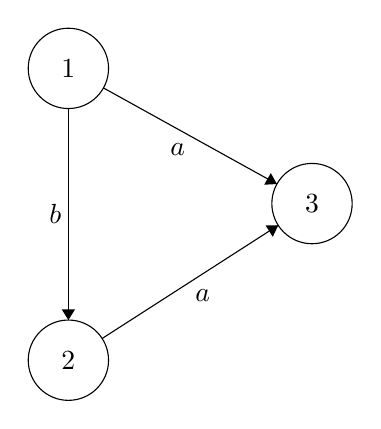
\begin{tikzpicture}[scale=0.17]
            \tikzstyle{every node}+=[inner sep=0pt]
            \draw [black] (17.2,-13.3) circle (3);
            \draw (17.2,-13.3) node {$1$};
            \draw [black] (17.2,-35.1) circle (3);
            \draw (17.2,-35.1) node {$2$};
            \draw [black] (35.4,-23.4) circle (3);
            \draw (35.4,-23.4) node {$3$};
            \draw [black] (19.82,-14.76) -- (32.78,-21.94);
            \fill [black] (32.78,-21.94) -- (32.32,-21.12) -- (31.83,-21.99);
            \draw (25.36,-18.85) node [below] {$a$};
            \draw [black] (17.2,-16.3) -- (17.2,-32.1);
            \fill [black] (17.2,-32.1) -- (17.7,-31.3) -- (16.7,-31.3);
            \draw (16.7,-24.2) node [left] {$b$};
            \draw [black] (19.72,-33.48) -- (32.88,-25.02);
            \fill [black] (32.88,-25.02) -- (31.93,-25.03) -- (32.47,-25.88);
            \draw (27.24,-29.75) node [below] {$a$};
        \end{tikzpicture}
        \label{ex-lab_tran_sys}
        \caption{A labelled transition system}
    \end{figure}

    In figure \ref{ex-lab_tran_sys} a labelled transition system is given where $\alpha(1) = \{(a,3),(b,2)\}$, $\alpha(2) = \{(a,3)\}$, $\alpha(3) = \varnothing$.
\end{example}

\begin{definition}
    A pointed $F$-coalgebra over a functor $F$ is a triple $(X, \alpha: X\to FX, x_0)$ where $X$ is the carrier as usual and $x_0$ is the \emph{base} or in our case an \emph{initial state}.
\end{definition}

\newpage
\section{Ranked Hypergraphs}
\begin{definition}
    A directed \emph{hypergraph} $(V,H)$ is a finite set of vertices $V$ and a set of \emph{hyperarcs} $H\subseteq V\times\P(V)$.
\end{definition}

\emph{Notation:} A directed hypergraph containing no cycles is a Directed Acyclic Hypergraph (DAH).

\begin{definition}
A \emph{ranked hypergraph} $(g, r, o, \L, A)$ consists of:
\begin{itemize}
\item A DAH $g$,
\item Finite sequences $r = (r_i)_{i\leq |r|}$, $o = (o_i)_{i\leq |o|}$ $r_i, o_i\in \P(V)$ denoting the root and variable interfaces. $o_i$ contains only maximal vertices. We refer to $(|r|, |o|)$ as the \emph{rank} of this graph.
\item An action set $A$ and a hyperarc labelling function $\L: H\to A$
\end{itemize}
\end{definition}
\emph{Notation:} In this thesis we often refer to ranked hypergraphs as just hypergraphs as we will only be working with this kind. $HG(n,m)$ is the set of ranked term hypergraphs of rank $(n,m)$

\begin{example}
    In figure \thref{fig:DAH-example} a ranked hypergraph is drawn. Left is the root interface, of rank 3, on the right is the output interface of rank 2. 

    The full definition of this graph is as follows
    \begin{itemize}
        \item $V = \{1,2,3,4,5,6\}$,
        \item $H = \{(1, \{4\}), (2, \{5,6\})\}$,
        \item $r = (\{1\}, \{2\}, \{3\})$, $o = (\{4\}, \{3,6\})$,
        \item $A = \{a,b\}$, $\L((1, \{4\})) = b$, $\L((2, \{5,6\})) = a$.
    \end{itemize}
    
    \begin{figure}[h]
    \centering
    \begin{tikzpicture}
		\node [style={gra_point}, label={above:1}] (0) at (-1, 1.5) {};
		\node [style={gra_point}, label={above:2}] (1) at (-1, 0) {};
		\node [style={gra_point}, label={above:4}] (3) at (1, 1.5) {};
		\node [style={int_point}] (5) at (-3, 1.5) {};
		\node [style={int_point}] (6) at (-3, 0) {};
		\node [style={int_point}] (7) at (-3, -1.75) {};
		\node [style={int_point}] (8) at (3.75, 1.25) {};
		\node [style={int_point}] (9) at (3.75, -1.25) {};
		\node [style={gra_point}, label={above:6}] (10) at (1, -0.75) {};
		\node [style={gra_point}, label={above:5}] (11) at (1, 0.5) {};
		\node [label={above:a}] (12) at (0, 0) {};
		\node [label={above:b}] (13) at (0, 1.5) {};
		\node [style={gra_point}, label={above:3}] (14) at (0, -1.75) {};
		\draw [style={int_edge}] (5) to (0);
		\draw (1) to (12.center);
		\draw [style={int_edge}] (7) to (14);
		\draw [style={int_edge}] (6) to (1);
		\draw [style={int_edge}] (9) to (14);
		\draw [style={int_edge}] (9) to (10);
		\draw [style={int_edge}] (8) to (3);
		\draw [style={gra_edge}] (0) to (3);
		\draw [style={gra_edge}] (12.center) to (11);
		\draw [style={gra_edge}] (12.center) to (10);
    \end{tikzpicture}
    \caption{A Directed Acyclic Hypergraph}
    \thlabel{fig:DAH-example}
\end{figure}
\end{example} % ranked hypergraph

\begin{definition}\thlabel{def_isomorphism}
Let $G,H\in HG(n,m)$ be ranked hypergraphs of equal rank $(n,m)$,

An \emph{isomorphism} between $G$ and $F$ is a bijection
\[
f : V^G \to V^F
\]
such that
\[
(u, U') \in H^G 
\iff
(f(u), f[U']) \in H^F
\]
\[
      v\in r^G_i \iff f(v)\in r^F_i \quad \forall i\leq n 
\]
\[
    v\in o^G_i \iff f(v)\in o^F_i \quad \forall i\leq m
\]
\end{definition} % ranked hypergraph isomorphism

\begin{remark}\thlabel{rem_rename}
    When proving a property which involves multiple hypergraphs, we can assume disjointness of vertex sets. But then the property will only hold up to isomorphism. This is because renaming of vertices is an isomorphism in the sense of \thref{def_isomorphism}.
\end{remark}

\subsection{Composition of ranked hypergraphs}
\begin{definition}\thlabel{def_seq_comp}
Let $G, F$ be hypergraphs such that $|o^G| = |r^F|$, their composition is defined as follows:
\begin{align}
    G\seq F = (g', r', i_F[o^F] \defeq (i_F[o_i^F])_{i\leq |o^F|}, \L^G\sqcup \L^F, A^G\cup A^F)
\end{align}

We obtain $g' = (V,H)$ by the following procedure:

Define 
\begin{align*}
    V = (V^G + V^F) \setminus i_G[\bigcup_{i\leq |o^G|}o^G_i]
\end{align*}

To get the hyperarcs we keep all elements but replace a vertex if it exists in an output, to do this neatly we define a pair of functions:

\[
\psi_{G,F}(v) := 
\begin{cases}
    i_F[\displaystyle\bigcup_{\substack{i\leq |o^G| \\ v \in o^G_i}} r^F_i] & \text{if } \exists i \leq |o^G| \text{ such that } v \in o^G_i \\
    \{i_G(v)\} & \text{else}
\end{cases}
\]

\[
\Psi_{G, F}(U') := \bigcup_{v \in U'} \psi_{G, F}(v)
\]

\[
H := \left\{ \left(i_G(u), \Psi_{G, F}(U')\right) : (u, U') \in H^G \right\} \cup i_F[H^F]
\]

So for all $i$, in each arc $v$ that ends in a vertex in $o_i^G$, we replace that vertex in the arc with $r_i^F$. 

And we obtain $r'$ by taking over the original $r^G$ and `connecting through' for vertices which are both minimal and maximal:
\begin{align*}
    r'_i = \Psi_{G, F}(r^G_i)
\end{align*}
\end{definition}

\begin{remark}\thlabel{rem_disj_seq_comp}
    When vertex sets are disjoint, we can simply take set union as coproduct. Which makes the inclusions identity maps.
\end{remark}

This composition allows for a left identity $id_n$ namely $id_n = ((\{1,2,\dots,n\}, \varnothing), (\{i\})_{i\in n}, (\{i\})_{i\in n})$.

\begin{example}
    Figure \ref{fig:composition} shows the sequential composition $G\seq F$. In this example it is visible that interface points give a handle on dependencies. For instance, as $4\in o_G$, and $7\in r_F$, in the final product $7$ is dependent on action $b$,
    \begin{figure}[H]
        \centering
        \begin{tikzpicture}
    		\node [style={gra_point}, label={above:1}] (0) at (-1, 1.5) {};
    		\node [style={gra_point}, label={above:2}] (1) at (-1, 0) {};
    		\node [style={gra_point}, label={above:4}] (3) at (1, 1.5) {};
    		\node [style={int_point}] (5) at (-3, 1.5) {};
    		\node [style={int_point}] (6) at (-3, 0) {};
    		\node [style={int_point}] (7) at (-3, -1.75) {};
    		\node [style={int_point}] (8) at (3.75, 1.25) {};
    		\node [style={int_point}] (9) at (3.75, -1.25) {};
    		\node [style={gra_point}, label={above:6}] (10) at (1, -0.75) {};
    		\node [style={gra_point}, label={above:5}] (11) at (1, 0.5) {};
    		\node [style=invisible, label={above:a}] (12) at (0, 0) {};
    		\node [style=invisible, label={above:b}] (13) at (0, 1.5) {};
    		\node [style={gra_point}, label={above:3}] (14) at (0, -1.75) {};
    		\node [style={int_point}] (15) at (5.25, 1.25) {};
    		\node [style={int_point}] (16) at (5.25, -1.25) {};
    		\node [style={gra_point}, label={above:7}] (17) at (7, 1.25) {};
    		\node [style={gra_point}, label={above:8}] (18) at (7, 0) {};
    		\node [style={gra_point}, label={above:9}] (19) at (7, -1.25) {};
    		\node [style={gra_point}, label={above:10}] (20) at (9.25, 1.25) {};
    		\node [style={gra_point}, label={above:11}] (21) at (9, -1.25) {};
    		\node [style={int_point}] (22) at (10.75, 1.25) {};
    		\node [style={int_point}] (23) at (10.75, -1.25) {};
    		\node [style=invisible, label={above:c}] (24) at (8, 1.25) {};
    		\node [style=invisible, label={below:a}] (25) at (8, 0.5) {};
    		\node [style=invisible, label={above:b}] (26) at (8, -1.25) {};
    		\node [style=invisible, label={above:\seq}] (27) at (4.5, -0.5) {};
    		\node [style={gra_point}, label={above:1}] (28) at (1.75, -3.5) {};
    		\node [style={gra_point}, label={above:2}] (29) at (1.75, -5) {};
    		\node [style={int_point}] (31) at (-0.25, -3.5) {};
    		\node [style={int_point}] (32) at (-0.25, -5) {};
    		\node [style={int_point}] (33) at (-0.25, -6.5) {};
    		\node [style={gra_point}, label={above:5}] (37) at (4.25, -4.25) {};
    		\node [style=invisible, label={above:a}] (38) at (3.25, -5) {};
    		\node [style=invisible, label={above:b}] (39) at (3.5, -3.5) {};
    		\node [style={gra_point}, label={above:7}] (43) at (5.5, -3.5) {};
    		\node [style={gra_point}, label={above:8}] (44) at (5.5, -5) {};
    		\node [style={gra_point}, label={above:9}] (45) at (5.5, -6.25) {};
    		\node [style={gra_point}, label={above:10}] (46) at (7.5, -3.5) {};
    		\node [style={gra_point}, label={above:11}] (47) at (7.5, -6.25) {};
    		\node [style={int_point}] (48) at (9.25, -3.5) {};
    		\node [style={int_point}] (49) at (9.25, -6.25) {};
    		\node [style=invisible, label={above:c}] (50) at (6.5, -3.5) {};
    		\node [style=invisible, label={below:a}] (51) at (6.25, -4.5) {};
    		\node [style=invisible, label={above:b}] (52) at (6.5, -6.25) {};
    		\node [style=invisible, label={above:=}] (53) at (-2, -5.5) {};
    		\draw [style={int_edge}] (5) to (0);
    		\draw (1) to (12.center);
    		\draw [style={int_edge}] (7) to (14);
    		\draw [style={int_edge}] (6) to (1);
    		\draw [style={int_edge}] (9) to (14);
    		\draw [style={int_edge}] (9) to (10);
    		\draw [style={int_edge}] (8) to (3);
    		\draw [style={gra_edge}] (0) to (3);
    		\draw [style={gra_edge}] (12.center) to (11);
    		\draw [style={gra_edge}] (12.center) to (10);
    		\draw [style={int_edge}] (15) to (17);
    		\draw [style={int_edge}] (16) to (18);
    		\draw [style={int_edge}] (16) to (19);
    		\draw [style={gra_edge}] (18) to (20);
    		\draw [style={gra_edge}] (17) to (20);
    		\draw [style={gra_edge}] (19) to (21);
    		\draw [style={int_edge}] (22) to (20);
    		\draw [style={int_edge}] (23) to (21);
    		\draw [style={int_edge}] (31) to (28);
    		\draw (29) to (38.center);
    		\draw [style={int_edge}] (32) to (29);
    		\draw [style={gra_edge}] (28) to (43);
    		\draw [style={gra_edge}] (38.center) to (37);
    		\draw [style={gra_edge}] (44) to (46);
    		\draw [style={gra_edge}] (43) to (46);
    		\draw [style={gra_edge}] (45) to (47);
    		\draw [style={int_edge}] (48) to (46);
    		\draw [style={int_edge}] (49) to (47);
    		\draw [style={int_edge}, bend right] (33) to (44);
    		\draw [style={int_edge}, bend right=15, looseness=1.25] (33) to (45);
    		\draw [style={gra_edge}] (38.center) to (44);
    		\draw [style={gra_edge}] (38.center) to (45);
        \end{tikzpicture}
        \caption{The composition of two ranked hypergraphs}
        \label{fig:composition}
    \end{figure}
\end{example}

\begin{lemma}\thlabel{lem:psieq}
    Let $G,K,F$ be DAH and $U\subseteq V^G$ a set of vertices, it holds that:
    \[
        \Psi_{G;K, F}\circ \Psi_{G, K}(U) \cong \Psi_{G, F;K}(U)
    \]
\end{lemma}

\begin{proof}
Let $G,K,F$ be DAH and $U\subseteq V^G$ a set of vertices. Assume disjoint vertex sets. 

We prove the lemma for a singleton, this then extends trivially to all subsets $U\subseteq V^G$. Let $v\in V^G$, we proceed by using the definitions:
    \begin{align*}
        \Psi_{G;K, F}\circ \psi_{G, K}(v) &= 
        \begin{cases}
            \{v\} & v\notin \cup_i o_i^G\\
            \Psi_{G;K, F}\left(\bigcup_{\substack{j \leq |r^K| \\ v \in o^G_j}} r^K_j\right) & \text{else}
        \end{cases}\\
        \intertext{Because both unions are finite we can exchange them: }
        &= 
        \begin{cases}
            \{v\} & v\notin \cup_i o_i^G\\
            \bigcup_{\substack{j \leq |r^K| \\ v \in o^G_j}} \Psi_{G;K, F} (r^K_j) & \text{else}\\
        \end{cases}\\
        \intertext{By definition $r^{K\seq F}_i \defeq \Psi_{K, F} (r^K_i)$ and hence}
        &=
        \begin{cases}
            \{v\} & v\notin \cup_i o_i^G\\
            \bigcup_{\substack{j\leq  |r^{K\seq F}| \\ v \in o^G_j}} r^{K\seq F}_j & \text{else}\\
        \end{cases}\\
        &= \psi_{G, K;F}(v)
    \end{align*}

    Taking unions of singletons then yields:
    \[
        \Psi_{K,F}\circ \Psi_{G, K}(U) = \Psi_{G,K;F}(U)
    \]

    By \thref{rem_rename} the equality holds up to isomorphism for all $G,K,F$, regardless of vertex sets.
\end{proof}

\begin{theorem}\thlabel{thm:assoc}
Let G,K,F be ranked hypergraphs. The following properties hold:
    \begin{enumerate}
        \item $G\seq(K\seq F) \cong (G\seq K) \seq F$
        \item $id_{|r^G|} \seq G \cong G$
    \end{enumerate}
\end{theorem} % associativity

\begin{proof}{$G\seq(K\seq F) \cong (G\seq K) \seq F$}\\
    Let $G,K,F$ be ranked hypergraphs with disjoint vertex sets. Use \thref{rem_disj_seq_comp}. It is clear from the definition that $(G \seq K) \seq F = G \seq (K \seq F)$ if and only if their graphs and root interfaces are equal.
         
    Let $r$, $r'$ be the root interfaces for $(G \seq K) \seq F$, $G \seq (K \seq F)$ respectively.  
    We expand the definition and use \thref{lem:psieq} to show that $r = r'$. Let $i\leq |r^G|$, we get:
    
    \begin{align*}
        r_i = \Psi_{r^F, o^k}(r^{G\seq K}_i) = \Psi_{r^F, o^k}(\Psi_{r^K, o^G}(r^G_i)) = \Psi_{r^{K\seq F}, o^G}(r_i) = r'_i\\
    \end{align*}

    Let $g = (V, H)$, $g' = (V', H')$ be the graphs for $(G \seq K) \seq F$, $G \seq (K \seq F)$ respectively.

    We expand the definition:
    \begin{gather*}
        V = (V^{G\seq K} + V^F) \setminus \bigcup_{i\leq |o^K|}o_i^K\\
        = (((V^G + V^K) \setminus \bigcup_{i\leq|o^G|}o^G_i) + V^F) \setminus \bigcup_{i\leq |o^K|}o_i^K
        \intertext{From disjointness of $V^G$, $V^K$, and $V^F$ we get}
        = (V^G + ((V^K + V^F) \setminus \bigcup_{i\leq|o^K|}o^K_i)) \setminus \bigcup_{i\leq|o^G|}o_i^G = V'
    \end{gather*}

    Lastly for the arcs:
    \begin{align*}
        H &= \left\{ \left(u, \Psi_{r^F, o^K}(U')\right) : (u, U') \in H^{G\seq K} \right\} \cup H^F\\
        &= \left\{ \left(u, \Psi_{r^F, o^K}(\Psi_{r^K, o^G}(U'))\right) : (u, U') \in H^G \right\}
        \cup \left\{ \left(u, \Psi_{r^F, o^K}(U')\right) : (u, U') \in H^K \right\} \cup H^F\\
        \intertext{By \thref{lem:psieq} we have}
        &= \left\{ \left(u, \Psi_{r^{F\seq K}, o^G}(U')\right) : (u, U') \in H^G \right\}
        \cup \left\{ \left(u, \Psi_{r^F, o^K}(U')\right) : (u, U') \in H^K \right\} \cup H^F\\
        &= \left\{ \left(u, \Psi_{r^{K \seq F}, o^G}(U')\right) : (u, U') \in H^G \right\} \cup H^{K \seq F}\\
        &= H'
    \end{align*}

    Which proves equality for disjoint graphs. Which in turn gives $G\seq(K\seq F) \cong (G\seq K) \seq F$ for any $G,K,F$ by using \thref{rem_rename}.
\end{proof}

\begin{proof}{$id_n \seq G \cong G$}\\
    Let $G$ be a ranked hypergraph with $|r^G| = n$ and \[id_n = ((\{1,2,\dots,n\}, \varnothing), (\{i\})_{i\in n}, (\{i\})_{i\in n})\] Assume disjoint vertex sets. Using remark \ref{rem_disj_seq_comp} we get:

    \[
        V = (\{1,2,\dots,n\}\cup V^G) \setminus \bigcup_{i\in n}\{i\} = V^G
    \]
    
    \[
        H = \left\{ \left(u, \Psi_{id_n\seq G}(U')\right) : (u, U') \in H^{id_n} \right\} \cup H^G = H^G
    \]

    \[
        \psi_{id_n\seq G} (i) = r^G_i \quad \forall i\in \{1,2,\dots,n\}
    \]

    Therefore 
    \[
        r'_i = \Psi_{id_n\seq G}(r^{id_n}_i) = \psi_{id_n\seq G}(i) = r^G_i
    \]

    From \ref{rem_rename} we conclude $id_n \seq G \cong G$ for any ranked hypergraph $G$.
\end{proof}

\subsection{Generating hypergraphs}

\begin{definition}
    First define the notion of predecessors of a vertex as:
    \begin{align*}
        \pred(v) = \{w\in V : \exists(w, U') \text{ s.t. } v\in U'\}
    \end{align*}

    Then we can define the depth of a vertex recursively
    \begin{align*}
        d: V \to \N, \quad d(v) = 
        \begin{cases}
            \max\{d(w) + 1 : w\in \pred(v)\} & \pred(v) \neq \varnothing\\
            0 & else 
        \end{cases}
    \end{align*}

    which extends to a notion of depth for an entire ranked hypergraph: \begin{align*}
        D(G) = \max\{d(v) : v\in V^G\}
    \end{align*}
\end{definition} % depth of hypergraph

\begin{theorem}\thlabel{thm_generator}
    The set of ranked hypergraphs is generated by the subset $$HG_1 \defeq \{G\in HG : D(G) \leq 1\}$$

    That is, for all $G\in HG$ there exists an $n\in \N_{\geq 1}$ and a sequence $(G_1, G_2, \dots, G_n)\in HG_1^n$, such that $G_1;G_2;\dots;G_n \cong G$
\end{theorem} % generator

\begin{proof}
    To prove this by induction we first need the following result:\\
    \emph{Claim:} for any hypergraph $G$ of depth $n \geq 2$ there exist hypergraphs $G_{1}\in HG$ with $D(G_1) = n-1$, $G_{2}\in HG_1$ such that $G \cong K\seq F$.

    First take $r^{1} = r$, $o^{2} = o$, $\L^{1} = \L^{2} = \L$, $A^{1} = A^{2} = A$.

    Then let
    \begin{align*}
        &V^1 = \{v\in V : d(v) \leq n-1 \text{ or } \exists w\in \pred(v) \text{ s.t. } d(w) < n-1\}\\
        &V^2 = \{v\in V : n-1 \leq d(v) \leq n\} \cup \bigcup_{i\leq |o^G|} o^G_i
    \end{align*}

    \begin{align*}
        &H^1 = \{(u,U')\in H : d(u) < n-1\}\\
        &H^2 = \{(u, U')\in H : d(u) = n-1\}
    \end{align*}

    Note that for all $(u,U') \in H_1$ we have $u\in V^1\setminus V^2$ because its degree is $< n-1$ and it isn't maximal and therefore not part of $o$. Furthermore, $(H^1, H^2)$ partitions $H$.

    Finally let $o^1 = r^2$ be any enumeration of $V^1\cap V^2$. 

    Let $i_1: V^1\to V^1 + V^2$, $i_2: V^2\to V^1 + V^2$ be the coproduct inclusions. We prove by construction of $G_1;G_2$ that the following function is an isomorphism
    \begin{align*}
        f: V\to (V^1 + V^2)\setminus i_1[\bigcup_{i\leq |o^1|}o^1_i], \quad f(v) = \begin{cases}
            i_1(v) & v\in V^1\setminus V^2\\
            i_2(v) & \text{else}
        \end{cases}
    \end{align*}

    % But first,
    % \begin{align*}
    %     V^{G_1;G_2} \defeq (V^1 + V^2) \setminus i_1[\bigcup_{i\leq |o^1|}o^1_i] = (V^1 + V^2) \setminus i_1[V^1\cap V^2] = f[V]
    % \end{align*}
    % which confirms that the function has the right domain and image.    

    First work out
    \begin{align*}
        \psi_{r^2, o^1}(v) &:= 
        \begin{cases}
            i_2[\displaystyle\bigcup_{\substack{i\leq |o^1| \\ v \in o^1_i}} r^2_i]& \text{if } \exists i \leq |o^1| \text{ such that } v \in o^1_i \\
            \{i_1(v)\} & \text{otherwise}
        \end{cases}\\
        \intertext{by $o^1=r^2$ we get}
        &=
        \begin{cases}
            \{i_2(v)\} & \text{if } v\in V^1\cap V^2\\
            \{i_1(v)\} & \text{otherwise}
        \end{cases}\\
        &= \{f(v)\} \quad \forall v\in V^1
    \end{align*}

    Therefore
    \begin{align*}
        H^{G_1;G_2} &\defeq \left\{ \left(i_1(u), f[U']\right) : (u, U') \in H^1 \right\} \cup i_2[H^2]\\
        &= \left\{ \left(f(u), f[U']\right) : (u, U') \in H^1 \right\} \cup \{(f(u), f[U'] : (u,U')\in H^2)\}\\
        &= \{(f(u), f[U'] : (u,U')\in H)\}\\
    \end{align*}

    and $r^{G_1;G_2} = (f[r^1_i])_{i\leq |r|} = (f[r_i])_{i\leq |r|}$, $o^{G_1;G_2} = (i_2[o_i^2])_{i\leq |o^F|} = (f[o_i])_{i\leq |o|}$

    Which proves $f$ to be an isomorphism. Hence we get $G_1;G_2 \cong G$ as claimed, furthermore from the chosen $H^1$ we obtain $D(G_1) = n-1$, $D(G_2) = 1 \implies G_2\in HG_1$.

    Now, let $G\in HG$ and assume $D(G) \leq 1$. This is trivially generated by $HG_1$ as $G\in HG_1$.

    Proceed by induction, assume all $G\in HG$ with $D(G) = n$ are generated by $HG_1$. Take $G\in HG$ with $D(G) = n+1$. From the just proven result there exist $G_1\in HG$, $G_2\in HG_1$ such that $D(G_1) = n$. Therefore there exists a sequence $(G_{11}, \dots, G_{1n}) \in $ such that $G_{11};\dots;G_{1n}\cong G_1$. Take as sequence $(G_{11}, \dots, G_{1n}, G_2)$, then $G_11; \dots; G_{1n}; G_2 \cong G_1; G_2 \cong G$. Thus all ranked hypergraphs of depth $n+1$ are generated by $HG$.

    By induction the statement holds for all $n$. Therefore $HG$ is generated by $HG_1$.
\end{proof}

% \begin{definition}
%     Let $G,F$ be hypergraphs such that $|o^G| \leq |r^F|$ we extend the notion of the sequential composition given by \ref{def_seq_comp} to asymmetric graph compositions. Write 
%     \begin{align*}
%         G\seq^+ F = (g', r', o^F, \L^G\sqcup \L^F, A^G\cup A^F)
%     \end{align*}

%     for the extended composition.

%     We obtain $g' = (V,H)$ by the following procedure:

%     \[
%         V \defeq (V^G + V^F) \setminus \bigcup_{i\leq |o^G|}o^G_i    
%     \]
    
%     \[
%         H \defeq \left\{ \left(U, \Psi_{r^F, o^G}(U')\right) : (U, U') \in H^G \right\} \cup H^F
%     \]

%     And do the same as $\seq$ for the interfaces except for the excess ones which we just copy:
%     \[
%         r'_i = 
%         \begin{cases}
%             \Psi_{r^F, o^G}(r^G_i) & i\leq |o^G|\\
%             r^F_i & else
%         \end{cases}
%     \]
% \end{definition} % extended seq composition

% By separation of cases we trivially extend theorem \ref{thm:assoc} to the following result:
% \begin{corollary}
%     $\seq^+$ is associative
% \end{corollary}
\newpage
\section{Simplicial sets over ranked term graphs}
From this point on, the necessary structures are less certain. We would like to encode the concurrency into the dimensions of our state space, which makes behaviour more predictable as we can control when and where changes in dimension happen. There are multiple ways to do this, one of them would be to keep track of the amount of interfaces. This gives a handle on the amount of possible dependencies, composition etcetera, this is the approach chosen for \thref{def:interface_simp}. Another, which is easier to parse semantically would be to keep track of the depth of the graph. 

\begin{definition}
    Let $V$ be the vertex set of a ranked hypergraph.\\
    We define the monoid $\M = (\P(V)^2, (\varnothing, \varnothing), \cup\times\cup)$. 
\end{definition}

From this monoid we define a simplicial set using the nerve construction.

\begin{definition}
    The \emph{nerve} $N(\M)$ of the monoid $\M$ is the simplicial set where:
    \begin{align*}
        N(\M)_n = \M^n\\
        d^{\M}_i(m_1,\dots,m_n) = 
        \begin{cases}
            (m_1,\dots,m_i \cup\times\cup m_{i+1}, \dots, m_n) & 0 < i < n\\
            (m_2,\dots, m_n) & i = 0\\
            (m_1,\dots,m_{n-1}) & i = n
        \end{cases}\\
        s^{\M}_i(m_1,\dots,m_n) = (m_1, \dots, m_i, (\varnothing, \varnothing), m_{i+1}, \dots, m_n)\\
    \end{align*}
\end{definition}

\begin{definition}\thlabel{def:interface_simp}
Define the simplicial set $\H$ by $\H_n = HG(n,n)$. With face and degeneracy maps:
\begin{align*}
    &d_i^{\H} ((g, (U_1, \dots, U_n), (W_1, W_2, \dots, W_n), \L, A))\\
    &\quad=\begin{cases}
        (g, (U_1, \dots, U_i\cup U_{i+1}, \dots U_n), (W_1, \dots, W_i\cup W_{i+1}, \dots W_n), \L, A) & 0 < i < n\\
        (g, (U_2, \dots, U_n), (W_1, W_2, \dots, W_n), \L, A) & i = 0\\
        (g, (U_1, \dots, U_{n-1}), (W_1, \dots, W_{n-1}), \L, A) & i = n
    \end{cases}\\
    \hspace{5pt}
    &s_i^{\H}((g, (U_1, \dots, U_n), (W_1, W_2, \dots, W_n), \L, A))\\
    &=\quad (g, (U_1, \dots U_i, \varnothing, U_{i+1}, \dots, U_n), (W_1, \dots W_i, \varnothing, W_{i+1}, \dots, W_n), \L, A)
\end{align*}
\end{definition}

\begin{lemma}
    $\H$ is indeed a simplicial set.
\end{lemma}

\begin{proof}
    Let $\pi_n: \H_n \to N(\M)_n$ be the projection onto the interfaces given by $\pi_n((g, r, o, \L, A)) = ((r_i, o_i))_{i\in [n]}$.

    \emph{Claim: } the following diagrams commute.
    \[
        \begin{tikzcd}
            \H_n \arrow{r}{d_i^{\H}} \arrow{d}{\pi_n} & \H_{n-1} \arrow{d}{\pi_{n-1}} \\
            N(\M)_n \arrow{r}{d_i^\M} & N(\M)_{n-1}
        \end{tikzcd}
        \quad
        \begin{tikzcd}
            \H_n \arrow{r}{s_j^{\H}} \arrow{d}{\pi_n} & \H_{n+1} \arrow{d}{\pi_{n+1}} \\
            N(\M)_n \arrow{r}{s_j^\M} & N(\M)_{n+1}
        \end{tikzcd}
    \]
    \begin{align*}
        \intertext{\textbf{Face maps} \newline $i = 0$:}
        &\pi_{n-1}(d_0^\mathcal{H}((g, (U_1, \ldots, U_n), (W_1, \ldots, W_n), \mathcal{L}, A))) \\
        &= \pi_{n-1}((g, (U_2, \ldots, U_n), (W_2, \ldots, W_n), \mathcal{L}, A)) \\
        &= ((U_2, W_2), \ldots, (U_n, W_n)) \\
        &= d_0^\mathcal{M}((U_1, W_1), \ldots, (U_n, W_n)) \\
        &= d_0^\mathcal{M}(\pi_n((g, (U_1, \ldots, U_n), (W_1, \ldots, W_n), \mathcal{L}, A))) \\
        \intertext{$0 < i < n$:}
        &\pi_{n-1}(d_i^\mathcal{H}((g, (U_1, \ldots, U_n), (W_1, \ldots, W_n), \mathcal{L}, A))) \\
        &= \pi_{n-1}((g, (U_1, \ldots, U_i \cup U_{i+1}, \ldots, U_n), (W_1, \ldots, W_i \cup W_{i+1}, \ldots, W_n), \mathcal{L}, A)) \\
        &= ((U_1, W_1), \ldots, (U_i \cup U_{i+1}, W_i \cup W_{i+1}), \ldots, (U_n, W_n)) \\
        &= d_i^\mathcal{M}((U_1, W_1), \ldots, (U_n, W_n)) \\
        &= d_i^\mathcal{M}(\pi_n((g, (U_1, \ldots, U_n), (W_1, \ldots, W_n), \mathcal{L}, A)))
        \intertext{$i = n$:}
        &\pi_{n-1}(d_n^\mathcal{H}((g, (U_1, \ldots, U_n), (W_1, \ldots, W_n), \mathcal{L}, A))) \\
        &= \pi_{n-1}((g, (U_1, \ldots, U_{n-1}), (W_1, \ldots, W_{n-1}), \mathcal{L}, A)) \\
        &= ((U_1, W_1), \ldots, (U_{n-1}, W_{n-1})) \\
        &= d_n^\mathcal{M}((U_1, W_1), \ldots, (U_n, W_n)) \\
        &= d_n^\mathcal{M}(\pi_n((g, (U_1, \ldots, U_n), (W_1, \ldots, W_n), \mathcal{L}, A)))
        \intertext{\textbf{Degeneracy maps}}
        &\pi_{n+1}(s_i^\mathcal{H}((g, (U_1, \ldots, U_n), (W_1, \ldots, W_n), \mathcal{L}, A))) \\
        &= \pi_{n+1}((g, (U_1, \ldots, U_i, \varnothing, U_{i+1}, \ldots, U_n), (W_1, \ldots, W_i, \varnothing, W_{i+1}, \ldots, W_n), \mathcal{L}, A)) \\
        &= ((U_1, W_1), \ldots, (U_i, W_i), (\varnothing, \varnothing), (U_{i+1}, W_{i+1}), \ldots, (U_n, W_n)) \\
        &= s_i^\mathcal{M}((U_1, W_1), \ldots, (U_n, W_n)) \\
        &= s_i^\mathcal{M}(\pi_n((g, (U_1, \ldots, U_n), (W_1, \ldots, W_n), \mathcal{L}, A)))
    \end{align*}

    Thus $\pi_n$ is a simplicial morphism. Therefore since $N(\M)$ is a simplicial set by definition the simplicial identities also hold for $d^{\H}$ and $s^{\H}$. Therefore $\H$ is a simplicial set.
\end{proof}

Note that for a given ranked hypergraph $G$ its underlying DAH $g$ is invariant under $d$ and $s$. This leads to the following result.

\begin{corollary}
    $\H^1 \defeq HG_1\cap \H$ is a subobject of $\H$. That is, $\H^1$ is a simplicial set with as face and degeneracy maps $d^{\H}$, respectively $s^{\H}$.
\end{corollary}

\begin{proof}
    $d^{\H}$, $s^{\H}$ already satisfy the simplicial identities. All that remains to be proven is that $\H^1$ is closed under them. Let $G\in \H^1_n$, then $F \defeq d^{\H}_i(G)$ has $g^F = g^G$ by definition of $d^{\H}$. Therefore $D(F) = D(G) = 1$ and hence $F\in \H^1_{n-1}$. Idem for $s^{\H}$. Thus $\H^1$ is a subobject of $\H$
\end{proof}
\newpage
\section{Towards coalgebraic behaviour}
For our setup a coalgebra with well-defined behaviour is not yet found. Therefore in this section we pose a potential coalgebra and a subsequent behaviour function, which has a few problems. Besides this we propose some solutions, which might be worth further investigation.

\subsection{The idea}
To add behaviour to the hypergraph simplicial set we define pointed F-coalgebras by the endofunctor

\begin{definition}\thlabel{def_endofunc}
    \begin{align*}
        F: sSet \to sSet, \quad FX = \Omega \times \finP(X \sqcup \uparrow X)^{HG_1}
    \end{align*}
\end{definition}

Through this definition we find out what a coalgebra does on our set. If we follow the repeated iteration of this coalgebra
\[
    X\xrightarrow{\alpha} FX \xrightarrow{F\alpha} FFX \xrightarrow{FF\alpha} \dots
\]

We get by definition of $F(f)$ that $\alpha$ gets recursively applied to the transitioned-to elements. This will look like

\begin{align*}
    \alpha(x_0) &= (0, \{g_{01}\mapsto x_{01}, g_{02}\mapsto x_{02}, \dots\})\\
    \implies \alpha\circ\alpha(x_0) &= (0, \{(g_{01}\mapsto (0, \{g_{011}\mapsto x_{011}, g_{012}\mapsto x_{012}\})),\\
    &\hspace{40pt}(g_{02}\mapsto (0, \{g_{021}\mapsto x_{021}, g_{022}\mapsto x_{022}\})), \dots\})
\end{align*}

Which is a tree structure with $x_0$ as root, $x_{01}, x_{02}, \dots$ as children etcetera. The transitions are through the hypergraphs.  In figure \ref{ex:coalg-tree} a tree is visualized for some coalgebra. Non-accepting states are red, and accepting states are indicated by a green node. Here $x_{012}$ is an accepting state.

\begin{figure}[H]
    \centering
    \begin{tikzpicture}[->, level distance=2cm,
            level 1/.style={sibling distance=4cm},
            level 2/.style={sibling distance=3cm},
            edge from parent node/.style={black},
            every node/.style={red}]
    \node (Root) {$x_0$}
        child {
            node {$x_{01}$}
            child { 
                node {$x_{011}$}
                child {
                    node {$\iddots\hspace{20pt}$}
                }
                child {
                    node {$\hspace{20pt}\ddots$}
                }
                edge from parent node[left, black] {$g_{011}$} 
            }
            child { 
                node [Green] {$x_{012}$}
                child {
                    node {$\vdots$}
                }
                edge from parent node[right, black] {$g_{012}$}
            }
            edge from parent node[left, black] {$g_{01}$}
        }
        child {
            node {$x_{02}$}
            child { 
                node {$x_{021}$}
                child {
                    node {$\vdots$}
                }
                edge from parent node[left, black] {$g_{021}$}
            }
            child { 
                node {$x_{022}$}
                child {
                    node {$\iddots\hspace{20pt}$}
                }
                child {
                    node {$\hspace{20pt}\ddots$}
                }
                edge from parent node[right, black] {$g_{022}$}
            }
            edge from parent node[right, black] {$g_{02}$}
        };
    \end{tikzpicture}
    \caption{Tree from iteration of some $F$-coalgebra}
    \label{ex:coalg-tree}
\end{figure}

\begin{definition}
    Let $(A, \vee, \bot)$ be a join-semilattice. We define the JSL morphism $\bigvee: \finP(A) \to A$ as the map making the following commute:

    \begin{center}
        \begin{tikzcd}
              A \arrow[d,"\eta"]\arrow[r,"\id_{A}"] & A \\
              \finP(A) \arrow[ur, swap, "\bigvee"]
        \end{tikzcd}
    \end{center}

    by lemma \ref{lem:free_jsl} $\finP(A)$ is the free JSL, hence $\bigvee$ exists and is unique.
\end{definition}

\begin{definition}
    Let $ev: A\times [A,B] \to B$, $(a, f)\mapsto f(a)$ be the evaluation morphism. We extend this to evaluate finite powersets by taking
    \begin{align*}
        \finP ev: \finP(A)\times [A,B] \to \finP(B)\\
        \finP ev(\{a_1, \dots, a_n\}, f) = \{f(a_1), \dots, f(a_n)\}
    \end{align*}
\end{definition}

To find out if a ranked hypergraph is part of a coalgebras language we split it up into parts of depth 1 using theorem \ref{thm_generator}. Which are then used left to right to transition between states. If any of the final states is accepting, the graph is part of the language.

To formalise this we define a behaviour function.

\begin{definition}
    Let $(X, c, x_0)$ be a pointed F-coalgebra of \ref{def_endofunc}. Define the so called \emph{behaviour function} as
    \begin{align*}
        \beh : \H \to [X, \Omega] \\
        \beh = \overline{(\beh_0, \beh_1)}
    \end{align*}
    Where $\beh$ is the inductive closure of $\beh_0, \beh_1$:\\
    \[
        \begin{array}{ll}
            \beh_0: \1 \to [X, \Omega] & \beh_0 = \lambda(\pi_1\circ c)\\
            \beh_1: HG_1\times [X, \Omega] \to [X, \Omega] & \beh_1 = \lambda_2 K
        \end{array}
    \]

    Where $K$ is a morphism defined by the following commuting diagram
    \begin{center}\label{dia_problems}
        \begin{tikzcd}
            HG_1\times X \times [X,\Omega]\arrow[r, "K"] \arrow[d, swap, "\widetilde{\pi_2\circ c} \times \id"] & \Omega\\
            \finP(X\sqcup \uparrow X)\times [X,\Omega] \arrow[r, "\finP ev"] & \finP(\Omega)\arrow[u, swap, "\bigvee"]
        \end{tikzcd}
    \end{center}
\end{definition}
\subsection{Current problems} The problems come in when looking at the bottom arrow of diagram \ref{dia_problems}. Here the carrier of the finite powerset in $\finP(X\sqcup \uparrow X)$ and the domain of the simplicial morphism in $[X,\Omega]$ aren't equal. Thus the use of the evaluation map $\finP ev$ isn't fully defined.

But intuitively it works. A simplicial map is a natural transformation, a family of morphisms such that there is one morphism for each $[n]\in \Delta$. So a potential solution is pointwise, for an $n$-cell in $X$ we transition to a finite set of $n$- and $n+1$-cells in $X\sqcup \uparrow X$. For any simplicial morphism $f: X\to S$ we have a function $f_n: X_n\to S_n$ for all $n$. Therefore we could evaluate all transitioned-to elements using a simplicial morphism with $X$ as domain.
\newpage

\section{Conclusions and Further Research}

\bibliographystyle{alphadin}
\bibliography{bibliography}
\addcontentsline{toc}{section}{References}
\end{document}